\documentclass[1p]{elsarticle_modified}
%\bibliographystyle{elsarticle-num}

%\usepackage[colorlinks]{hyperref}
%\usepackage{abbrmath_seonhwa} %\Abb, \Ascr, \Acal ,\Abf, \Afrak
\usepackage{amsfonts}
\usepackage{amssymb}
\usepackage{amsmath}
\usepackage{amsthm}
\usepackage{scalefnt}
\usepackage{amsbsy}
\usepackage{kotex}
\usepackage{caption}
\usepackage{subfig}
\usepackage{color}
\usepackage{graphicx}
\usepackage{xcolor} %% white, black, red, green, blue, cyan, magenta, yellow
\usepackage{float}
\usepackage{setspace}
\usepackage{hyperref}

\usepackage{tikz}
\usetikzlibrary{arrows}

\usepackage{multirow}
\usepackage{array} % fixed length table
\usepackage{hhline}

%%%%%%%%%%%%%%%%%%%%%
\makeatletter
\renewcommand*\env@matrix[1][\arraystretch]{%
	\edef\arraystretch{#1}%
	\hskip -\arraycolsep
	\let\@ifnextchar\new@ifnextchar
	\array{*\c@MaxMatrixCols c}}
\makeatother %https://tex.stackexchange.com/questions/14071/how-can-i-increase-the-line-spacing-in-a-matrix
%%%%%%%%%%%%%%%

\usepackage[normalem]{ulem}

\newcommand{\msout}[1]{\ifmmode\text{\sout{\ensuremath{#1}}}\else\sout{#1}\fi}
%SOURCE: \msout is \stkout macro in https://tex.stackexchange.com/questions/20609/strikeout-in-math-mode

\newcommand{\cancel}[1]{
	\ifmmode
	{\color{red}\msout{#1}}
	\else
	{\color{red}\sout{#1}}
	\fi
}

\newcommand{\add}[1]{
	{\color{blue}\uwave{#1}}
}

\newcommand{\replace}[2]{
	\ifmmode
	{\color{red}\msout{#1}}{\color{blue}\uwave{#2}}
	\else
	{\color{red}\sout{#1}}{\color{blue}\uwave{#2}}
	\fi
}

\newcommand{\Sol}{\mathcal{S}} %segment
\newcommand{\D}{D} %diagram
\newcommand{\A}{\mathcal{A}} %arc


%%%%%%%%%%%%%%%%%%%%%%%%%%%%%5 test

\def\sl{\operatorname{\textup{SL}}(2,\Cbb)}
\def\psl{\operatorname{\textup{PSL}}(2,\Cbb)}
\def\quan{\mkern 1mu \triangleright \mkern 1mu}

\theoremstyle{definition}
\newtheorem{thm}{Theorem}[section]
\newtheorem{prop}[thm]{Proposition}
\newtheorem{lem}[thm]{Lemma}
\newtheorem{ques}[thm]{Question}
\newtheorem{cor}[thm]{Corollary}
\newtheorem{defn}[thm]{Definition}
\newtheorem{exam}[thm]{Example}
\newtheorem{rmk}[thm]{Remark}
\newtheorem{alg}[thm]{Algorithm}

\newcommand{\I}{\sqrt{-1}}
\begin{document}

%\begin{frontmatter}
%
%\title{Boundary parabolic representations of knots up to 8 crossings}
%
%%% Group authors per affiliation:
%\author{Yunhi Cho} 
%\address{Department of Mathematics, University of Seoul, Seoul, Korea}
%\ead{yhcho@uos.ac.kr}
%
%
%\author{Seonhwa Kim} %\fnref{s_kim}}
%\address{Center for Geometry and Physics, Institute for Basic Science, Pohang, 37673, Korea}
%\ead{ryeona17@ibs.re.kr}
%
%\author{Hyuk Kim}
%\address{Department of Mathematical Sciences, Seoul National University, Seoul 08826, Korea}
%\ead{hyukkim@snu.ac.kr}
%
%\author{Seokbeom Yoon}
%\address{Department of Mathematical Sciences, Seoul National University, Seoul, 08826,  Korea}
%\ead{sbyoon15@snu.ac.kr}
%
%\begin{abstract}
%We find all boundary parabolic representation of knots up to 8 crossings.
%
%\end{abstract}
%\begin{keyword}
%    \MSC[2010] 57M25 
%\end{keyword}
%
%\end{frontmatter}

%\linenumbers
%\tableofcontents
%
\newcommand\colored[1]{\textcolor{white}{\rule[-0.35ex]{0.8em}{1.4ex}}\kern-0.8em\color{red} #1}%
%\newcommand\colored[1]{\textcolor{white}{ #1}\kern-2.17ex	\textcolor{white}{ #1}\kern-1.81ex	\textcolor{white}{ #1}\kern-2.15ex\color{red}#1	}

{\Large $\underline{12n_{0280}~(K12n_{0280})}$}

\setlength{\tabcolsep}{10pt}
\renewcommand{\arraystretch}{1.6}
\vspace{1cm}\begin{tabular}{m{100pt}>{\centering\arraybackslash}m{274pt}}
\multirow{5}{120pt}{
	\centering
	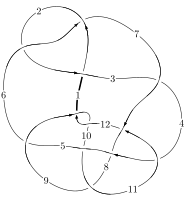
\includegraphics[width=112pt]{../../../GIT/diagram.site/Diagrams/png/2369_12n_0280.png}\\
\ \ \ A knot diagram\footnotemark}&
\allowdisplaybreaks
\textbf{Linearized knot diagam} \\
\cline{2-2}
 &
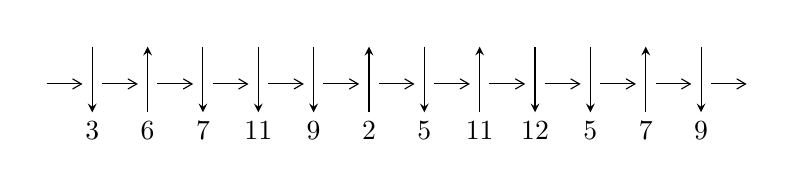
\begin{tikzpicture}[x=20pt, y=17pt]
	% nodes
	\node (C0) at (0, 0) {};
	\node (C1) at (1, 0) {};
	\node (C1U) at (1, +1) {};
	\node (C1D) at (1, -1) {3};

	\node (C2) at (2, 0) {};
	\node (C2U) at (2, +1) {};
	\node (C2D) at (2, -1) {6};

	\node (C3) at (3, 0) {};
	\node (C3U) at (3, +1) {};
	\node (C3D) at (3, -1) {7};

	\node (C4) at (4, 0) {};
	\node (C4U) at (4, +1) {};
	\node (C4D) at (4, -1) {11};

	\node (C5) at (5, 0) {};
	\node (C5U) at (5, +1) {};
	\node (C5D) at (5, -1) {9};

	\node (C6) at (6, 0) {};
	\node (C6U) at (6, +1) {};
	\node (C6D) at (6, -1) {2};

	\node (C7) at (7, 0) {};
	\node (C7U) at (7, +1) {};
	\node (C7D) at (7, -1) {5};

	\node (C8) at (8, 0) {};
	\node (C8U) at (8, +1) {};
	\node (C8D) at (8, -1) {11};

	\node (C9) at (9, 0) {};
	\node (C9U) at (9, +1) {};
	\node (C9D) at (9, -1) {12};

	\node (C10) at (10, 0) {};
	\node (C10U) at (10, +1) {};
	\node (C10D) at (10, -1) {5};

	\node (C11) at (11, 0) {};
	\node (C11U) at (11, +1) {};
	\node (C11D) at (11, -1) {7};

	\node (C12) at (12, 0) {};
	\node (C12U) at (12, +1) {};
	\node (C12D) at (12, -1) {9};
	\node (C13) at (13, 0) {};

	% arrows
	\draw[->,>={angle 60}]
	(C0) edge (C1) (C1) edge (C2) (C2) edge (C3) (C3) edge (C4) (C4) edge (C5) (C5) edge (C6) (C6) edge (C7) (C7) edge (C8) (C8) edge (C9) (C9) edge (C10) (C10) edge (C11) (C11) edge (C12) (C12) edge (C13) ;	\draw[->,>=stealth]
	(C1U) edge (C1D) (C2D) edge (C2U) (C3U) edge (C3D) (C4U) edge (C4D) (C5U) edge (C5D) (C6D) edge (C6U) (C7U) edge (C7D) (C8D) edge (C8U) (C9U) edge (C9D) (C10U) edge (C10D) (C11D) edge (C11U) (C12U) edge (C12D) ;
	\end{tikzpicture} \\
\hhline{~~} \\& 
\textbf{Solving Sequence} \\ \cline{2-2} 
 &
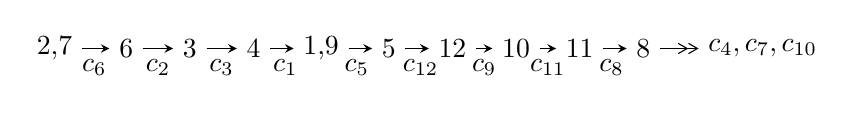
\begin{tikzpicture}[x=23pt, y=7pt]
	% node
	\node (A0) at (-1/8, 0) {2,7};
	\node (A1) at (1, 0) {6};
	\node (A2) at (2, 0) {3};
	\node (A3) at (3, 0) {4};
	\node (A4) at (65/16, 0) {1,9};
	\node (A5) at (41/8, 0) {5};
	\node (A6) at (49/8, 0) {12};
	\node (A7) at (57/8, 0) {10};
	\node (A8) at (65/8, 0) {11};
	\node (A9) at (73/8, 0) {8};
	\node (C1) at (1/2, -1) {$c_{6}$};
	\node (C2) at (3/2, -1) {$c_{2}$};
	\node (C3) at (5/2, -1) {$c_{3}$};
	\node (C4) at (7/2, -1) {$c_{1}$};
	\node (C5) at (37/8, -1) {$c_{5}$};
	\node (C6) at (45/8, -1) {$c_{12}$};
	\node (C7) at (53/8, -1) {$c_{9}$};
	\node (C8) at (61/8, -1) {$c_{11}$};
	\node (C9) at (69/8, -1) {$c_{8}$};
	\node (A10) at (11, 0) {$c_{4},c_{7},c_{10}$};

	% edge
	\draw[->,>=stealth]	
	(A0) edge (A1) (A1) edge (A2) (A2) edge (A3) (A3) edge (A4) (A4) edge (A5) (A5) edge (A6) (A6) edge (A7) (A7) edge (A8) (A8) edge (A9) ;
	\draw[->>,>={angle 60}]	
	(A9) edge (A10);
\end{tikzpicture} \\ 

\end{tabular} \\

\footnotetext{
The image of knot diagram is generated by the software ``\textbf{Draw programme}" developed by Andrew Bartholomew(\url{http://www.layer8.co.uk/maths/draw/index.htm\#Running-draw}), where we modified some parts for our purpose(\url{https://github.com/CATsTAILs/LinksPainter}).
}\phantom \\ \newline 
\centering \textbf{Ideals for irreducible components\footnotemark of $X_{\text{par}}$} 
 
\begin{align*}
I^u_{1}&=\langle 
- u^{18}+4 u^{17}+\cdots+b-1,\;- u^{19}+5 u^{18}+\cdots+2 a+4,\;u^{20}-5 u^{19}+\cdots-10 u+2\rangle \\
I^u_{2}&=\langle 
u^9+2 u^8+4 u^7+4 u^6+5 u^5+4 u^4+4 u^3+2 u^2+b+u+1,\\
\phantom{I^u_{2}}&\phantom{= \langle  }- u^{10}-4 u^9-7 u^8-10 u^7-9 u^6-11 u^5-10 u^4-8 u^3-4 u^2+2 a-3 u-4,\\
\phantom{I^u_{2}}&\phantom{= \langle  }u^{11}+2 u^{10}+5 u^9+6 u^8+9 u^7+9 u^6+10 u^5+8 u^4+6 u^3+5 u^2+2 u+2\rangle \\
I^u_{3}&=\langle 
- u^7 a-3 u^5 a- u^6+u^4 a-4 u^3 a-2 u^4+u^2 a+u^3-2 a u- u^2+b+a+u+1,\\
\phantom{I^u_{3}}&\phantom{= \langle  }-2 u^7 a+5 u^7+\cdots- a-4,\;u^8+u^7+3 u^6+2 u^5+3 u^4+2 u^3-1\rangle \\
\\
\end{align*}
\raggedright * 3 irreducible components of $\dim_{\mathbb{C}}=0$, with total 47 representations.\\
\footnotetext{All coefficients of polynomials are rational numbers. But the coefficients are sometimes approximated in decimal forms when there is not enough margin.}
\newpage
\renewcommand{\arraystretch}{1}
\centering \section*{I. $I^u_{1}= \langle - u^{18}+4 u^{17}+\cdots+b-1,\;- u^{19}+5 u^{18}+\cdots+2 a+4,\;u^{20}-5 u^{19}+\cdots-10 u+2 \rangle$}
\flushleft \textbf{(i) Arc colorings}\\
\begin{tabular}{m{7pt} m{180pt} m{7pt} m{180pt} }
\flushright $a_{2}=$&$\begin{pmatrix}0\\u\end{pmatrix}$ \\
\flushright $a_{7}=$&$\begin{pmatrix}1\\0\end{pmatrix}$ \\
\flushright $a_{6}=$&$\begin{pmatrix}1\\u^2\end{pmatrix}$ \\
\flushright $a_{3}=$&$\begin{pmatrix}u\\u^3+u\end{pmatrix}$ \\
\flushright $a_{4}=$&$\begin{pmatrix}- u^3\\u^3+u\end{pmatrix}$ \\
\flushright $a_{1}=$&$\begin{pmatrix}u^3\\u^5+u^3+u\end{pmatrix}$ \\
\flushright $a_{9}=$&$\begin{pmatrix}\frac{1}{2} u^{19}-\frac{5}{2} u^{18}+\cdots+10 u-2\\u^{18}-4 u^{17}+\cdots-3 u+1\end{pmatrix}$ \\
\flushright $a_{5}=$&$\begin{pmatrix}\frac{3}{2} u^{19}-\frac{13}{2} u^{18}+\cdots+u+1\\- u^{18}+5 u^{17}+\cdots+11 u-3\end{pmatrix}$ \\
\flushright $a_{12}=$&$\begin{pmatrix}-\frac{3}{2} u^{19}+\frac{13}{2} u^{18}+\cdots-7 u+1\\u^{19}-4 u^{18}+\cdots+5 u-1\end{pmatrix}$ \\
\flushright $a_{10}=$&$\begin{pmatrix}2 u^{19}-10 u^{18}+\cdots+13 u-2\\-2 u^{19}+8 u^{18}+\cdots-9 u+2\end{pmatrix}$ \\
\flushright $a_{11}=$&$\begin{pmatrix}-\frac{5}{2} u^{19}+\frac{21}{2} u^{18}+\cdots-12 u+2\\u^{19}-4 u^{18}+\cdots+5 u-1\end{pmatrix}$ \\
\flushright $a_{8}=$&$\begin{pmatrix}\frac{1}{2} u^{19}-\frac{1}{2} u^{18}+\cdots- u+1\\u^{19}-4 u^{18}+\cdots+4 u-1\end{pmatrix}$\\&\end{tabular}
\flushleft \textbf{(ii) Obstruction class $= -1$}\\~\\
\flushleft \textbf{(iii) Cusp Shapes $= -3 u^{19}+14 u^{18}-49 u^{17}+118 u^{16}-238 u^{15}+405 u^{14}-622 u^{13}+886 u^{12}-1180 u^{11}+1475 u^{10}-1689 u^9+1761 u^8-1647 u^7+1374 u^6-1015 u^5+655 u^4-363 u^3+170 u^2-66 u+12$}\\~\\
\newpage\renewcommand{\arraystretch}{1}
\flushleft \textbf{(iv) u-Polynomials at the component}\newline \\
\begin{tabular}{m{50pt}|m{274pt}}
Crossings & \hspace{64pt}u-Polynomials at each crossing \\
\hline $$\begin{aligned}c_{1}\end{aligned}$$&$\begin{aligned}
&u^{20}+11 u^{19}+\cdots+36 u+4
\end{aligned}$\\
\hline $$\begin{aligned}c_{2},c_{6}\end{aligned}$$&$\begin{aligned}
&u^{20}-5 u^{19}+\cdots-10 u+2
\end{aligned}$\\
\hline $$\begin{aligned}c_{3}\end{aligned}$$&$\begin{aligned}
&u^{20}+5 u^{19}+\cdots-10 u+10
\end{aligned}$\\
\hline $$\begin{aligned}c_{4},c_{7},c_{10}\end{aligned}$$&$\begin{aligned}
&u^{20}+15 u^{18}+\cdots+2 u+1
\end{aligned}$\\
\hline $$\begin{aligned}c_{5}\end{aligned}$$&$\begin{aligned}
&u^{20}+u^{19}+\cdots+u+1
\end{aligned}$\\
\hline $$\begin{aligned}c_{8}\end{aligned}$$&$\begin{aligned}
&u^{20}+11 u^{19}+\cdots+10 u+10
\end{aligned}$\\
\hline $$\begin{aligned}c_{9},c_{12}\end{aligned}$$&$\begin{aligned}
&u^{20}-3 u^{19}+\cdots+3 u+1
\end{aligned}$\\
\hline $$\begin{aligned}c_{11}\end{aligned}$$&$\begin{aligned}
&u^{20}-19 u^{19}+\cdots-2304 u+256
\end{aligned}$\\
\hline
\end{tabular}\\~\\
\newpage\renewcommand{\arraystretch}{1}
\flushleft \textbf{(v) Riley Polynomials at the component}\newline \\
\begin{tabular}{m{50pt}|m{274pt}}
Crossings & \hspace{64pt}Riley Polynomials at each crossing \\
\hline $$\begin{aligned}c_{1}\end{aligned}$$&$\begin{aligned}
&y^{20}- y^{19}+\cdots-208 y+16
\end{aligned}$\\
\hline $$\begin{aligned}c_{2},c_{6}\end{aligned}$$&$\begin{aligned}
&y^{20}+11 y^{19}+\cdots+36 y+4
\end{aligned}$\\
\hline $$\begin{aligned}c_{3}\end{aligned}$$&$\begin{aligned}
&y^{20}-13 y^{19}+\cdots+1940 y+100
\end{aligned}$\\
\hline $$\begin{aligned}c_{4},c_{7},c_{10}\end{aligned}$$&$\begin{aligned}
&y^{20}+30 y^{19}+\cdots+4 y+1
\end{aligned}$\\
\hline $$\begin{aligned}c_{5}\end{aligned}$$&$\begin{aligned}
&y^{20}-19 y^{19}+\cdots+7 y+1
\end{aligned}$\\
\hline $$\begin{aligned}c_{8}\end{aligned}$$&$\begin{aligned}
&y^{20}-3 y^{19}+\cdots+1460 y+100
\end{aligned}$\\
\hline $$\begin{aligned}c_{9},c_{12}\end{aligned}$$&$\begin{aligned}
&y^{20}-11 y^{19}+\cdots+11 y+1
\end{aligned}$\\
\hline $$\begin{aligned}c_{11}\end{aligned}$$&$\begin{aligned}
&y^{20}-9 y^{19}+\cdots+524288 y+65536
\end{aligned}$\\
\hline
\end{tabular}\\~\\
\newpage\flushleft \textbf{(vi) Complex Volumes and Cusp Shapes}
$$\begin{array}{c|c|c}  
\text{Solutions to }I^u_{1}& \I (\text{vol} + \sqrt{-1}CS) & \text{Cusp shape}\\
 \hline 
\begin{aligned}
u &= \phantom{-}0.988466 + 0.164208 I \\
a &= \phantom{-}0.083650 - 0.252088 I \\
b &= -1.31829 - 0.86406 I\end{aligned}
 & \phantom{-}3.16459 - 7.53851 I & -1.81526 + 4.10532 I \\ \hline\begin{aligned}
u &= \phantom{-}0.988466 - 0.164208 I \\
a &= \phantom{-}0.083650 + 0.252088 I \\
b &= -1.31829 + 0.86406 I\end{aligned}
 & \phantom{-}3.16459 + 7.53851 I & -1.81526 - 4.10532 I \\ \hline\begin{aligned}
u &= -0.230979 + 0.893127 I \\
a &= -1.51428 + 0.24987 I \\
b &= \phantom{-}0.618322 + 1.140400 I\end{aligned}
 & -0.82008 - 3.37374 I & -7.04529 + 0.08324 I \\ \hline\begin{aligned}
u &= -0.230979 - 0.893127 I \\
a &= -1.51428 - 0.24987 I \\
b &= \phantom{-}0.618322 - 1.140400 I\end{aligned}
 & -0.82008 + 3.37374 I & -7.04529 - 0.08324 I \\ \hline\begin{aligned}
u &= \phantom{-}0.743178 + 0.313816 I \\
a &= \phantom{-}0.040715 + 0.499230 I \\
b &= \phantom{-}0.715480 - 0.112619 I\end{aligned}
 & -0.854263 + 0.828569 I & -4.29561 - 2.11881 I \\ \hline\begin{aligned}
u &= \phantom{-}0.743178 - 0.313816 I \\
a &= \phantom{-}0.040715 - 0.499230 I \\
b &= \phantom{-}0.715480 + 0.112619 I\end{aligned}
 & -0.854263 - 0.828569 I & -4.29561 + 2.11881 I \\ \hline\begin{aligned}
u &= \phantom{-}0.348476 + 1.207610 I \\
a &= -1.77185 - 0.05613 I \\
b &= \phantom{-}1.221280 - 0.316490 I\end{aligned}
 & -5.09486 + 4.27767 I & -6.93870 - 3.93528 I \\ \hline\begin{aligned}
u &= \phantom{-}0.348476 - 1.207610 I \\
a &= -1.77185 + 0.05613 I \\
b &= \phantom{-}1.221280 + 0.316490 I\end{aligned}
 & -5.09486 - 4.27767 I & -6.93870 + 3.93528 I \\ \hline\begin{aligned}
u &= -0.904379 + 0.906046 I \\
a &= -0.071879 - 0.437712 I \\
b &= -0.847385 - 0.116530 I\end{aligned}
 & \phantom{-}8.73338 - 3.30325 I & -7.62069 + 4.42366 I \\ \hline\begin{aligned}
u &= -0.904379 - 0.906046 I \\
a &= -0.071879 + 0.437712 I \\
b &= -0.847385 + 0.116530 I\end{aligned}
 & \phantom{-}8.73338 + 3.30325 I & -7.62069 - 4.42366 I\\
 \hline 
 \end{array}$$\newpage$$\begin{array}{c|c|c}  
\text{Solutions to }I^u_{1}& \I (\text{vol} + \sqrt{-1}CS) & \text{Cusp shape}\\
 \hline 
\begin{aligned}
u &= -0.130781 + 0.697014 I \\
a &= \phantom{-}1.214520 + 0.459557 I \\
b &= \phantom{-}0.132234 - 0.751539 I\end{aligned}
 & -0.259969 + 1.114940 I & -6.76006 - 5.17901 I \\ \hline\begin{aligned}
u &= -0.130781 - 0.697014 I \\
a &= \phantom{-}1.214520 - 0.459557 I \\
b &= \phantom{-}0.132234 + 0.751539 I\end{aligned}
 & -0.259969 - 1.114940 I & -6.76006 + 5.17901 I \\ \hline\begin{aligned}
u &= \phantom{-}0.590387 + 1.171510 I \\
a &= -0.831475 - 0.979178 I \\
b &= \phantom{-}0.850680 - 0.233951 I\end{aligned}
 & -3.33496 + 4.34846 I & -6.57341 - 3.74600 I \\ \hline\begin{aligned}
u &= \phantom{-}0.590387 - 1.171510 I \\
a &= -0.831475 + 0.979178 I \\
b &= \phantom{-}0.850680 + 0.233951 I\end{aligned}
 & -3.33496 - 4.34846 I & -6.57341 + 3.74600 I \\ \hline\begin{aligned}
u &= \phantom{-}0.181642 + 0.634443 I \\
a &= \phantom{-}0.754937 + 0.401077 I \\
b &= \phantom{-}0.044656 - 0.325945 I\end{aligned}
 & -0.338993 + 1.073370 I & -4.95066 - 6.25444 I \\ \hline\begin{aligned}
u &= \phantom{-}0.181642 - 0.634443 I \\
a &= \phantom{-}0.754937 - 0.401077 I \\
b &= \phantom{-}0.044656 + 0.325945 I\end{aligned}
 & -0.338993 - 1.073370 I & -4.95066 + 6.25444 I \\ \hline\begin{aligned}
u &= \phantom{-}0.564854 + 1.265020 I \\
a &= \phantom{-}1.91175 + 0.60844 I \\
b &= -1.44189 + 1.06169 I\end{aligned}
 & -0.23167 + 13.11790 I & -4.38679 - 6.82889 I \\ \hline\begin{aligned}
u &= \phantom{-}0.564854 - 1.265020 I \\
a &= \phantom{-}1.91175 - 0.60844 I \\
b &= -1.44189 - 1.06169 I\end{aligned}
 & -0.23167 - 13.11790 I & -4.38679 + 6.82889 I \\ \hline\begin{aligned}
u &= \phantom{-}0.349135 + 1.341000 I \\
a &= \phantom{-}1.18393 + 0.98393 I \\
b &= -1.47508 - 0.55967 I\end{aligned}
 & -1.78563 - 2.89136 I & -6.11353 + 1.76882 I \\ \hline\begin{aligned}
u &= \phantom{-}0.349135 - 1.341000 I \\
a &= \phantom{-}1.18393 - 0.98393 I \\
b &= -1.47508 + 0.55967 I\end{aligned}
 & -1.78563 + 2.89136 I & -6.11353 - 1.76882 I\\
 \hline 
 \end{array}$$\newpage\newpage\renewcommand{\arraystretch}{1}
\centering \section*{II. $I^u_{2}= \langle u^9+2 u^8+\cdots+b+1,\;- u^{10}-4 u^9+\cdots+2 a-4,\;u^{11}+2 u^{10}+\cdots+2 u+2 \rangle$}
\flushleft \textbf{(i) Arc colorings}\\
\begin{tabular}{m{7pt} m{180pt} m{7pt} m{180pt} }
\flushright $a_{2}=$&$\begin{pmatrix}0\\u\end{pmatrix}$ \\
\flushright $a_{7}=$&$\begin{pmatrix}1\\0\end{pmatrix}$ \\
\flushright $a_{6}=$&$\begin{pmatrix}1\\u^2\end{pmatrix}$ \\
\flushright $a_{3}=$&$\begin{pmatrix}u\\u^3+u\end{pmatrix}$ \\
\flushright $a_{4}=$&$\begin{pmatrix}- u^3\\u^3+u\end{pmatrix}$ \\
\flushright $a_{1}=$&$\begin{pmatrix}u^3\\u^5+u^3+u\end{pmatrix}$ \\
\flushright $a_{9}=$&$\begin{pmatrix}\frac{1}{2} u^{10}+2 u^9+\cdots+\frac{3}{2} u+2\\- u^9-2 u^8-4 u^7-4 u^6-5 u^5-4 u^4-4 u^3-2 u^2- u-1\end{pmatrix}$ \\
\flushright $a_{5}=$&$\begin{pmatrix}-\frac{5}{2} u^{10}-4 u^9+\cdots-\frac{11}{2} u+1\\u^{10}+2 u^9+4 u^8+5 u^7+6 u^6+7 u^5+6 u^4+5 u^3+3 u^2+3 u+1\end{pmatrix}$ \\
\flushright $a_{12}=$&$\begin{pmatrix}-\frac{1}{2} u^{10}-2 u^9+\cdots-\frac{5}{2} u-3\\u^5+u^4+2 u^3+u^2+u+1\end{pmatrix}$ \\
\flushright $a_{10}=$&$\begin{pmatrix}u^{10}+5 u^9+9 u^8+15 u^7+15 u^6+19 u^5+17 u^4+15 u^3+9 u^2+6 u+6\\- u^9-2 u^8-4 u^7-4 u^6-5 u^5-4 u^4-4 u^3-2 u^2- u-2\end{pmatrix}$ \\
\flushright $a_{11}=$&$\begin{pmatrix}-\frac{1}{2} u^{10}-2 u^9+\cdots-\frac{7}{2} u-4\\u^5+u^4+2 u^3+u^2+u+1\end{pmatrix}$ \\
\flushright $a_{8}=$&$\begin{pmatrix}\frac{3}{2} u^{10}+7 u^9+\cdots+\frac{19}{2} u+11\\- u^9-2 u^8-4 u^7-4 u^6-6 u^5-5 u^4-6 u^3-3 u^2-2 u-3\end{pmatrix}$\\&\end{tabular}
\flushleft \textbf{(ii) Obstruction class $= 1$}\\~\\
\flushleft \textbf{(iii) Cusp Shapes $= - u^{10}-6 u^9-12 u^8-23 u^7-27 u^6-31 u^5-30 u^4-25 u^3-20 u^2-10 u-12$}\\~\\
\newpage\renewcommand{\arraystretch}{1}
\flushleft \textbf{(iv) u-Polynomials at the component}\newline \\
\begin{tabular}{m{50pt}|m{274pt}}
Crossings & \hspace{64pt}u-Polynomials at each crossing \\
\hline $$\begin{aligned}c_{1}\end{aligned}$$&$\begin{aligned}
&u^{11}-6 u^{10}+\cdots-16 u+4
\end{aligned}$\\
\hline $$\begin{aligned}c_{2}\end{aligned}$$&$\begin{aligned}
&u^{11}-2 u^{10}+5 u^9-6 u^8+9 u^7-9 u^6+10 u^5-8 u^4+6 u^3-5 u^2+2 u-2
\end{aligned}$\\
\hline $$\begin{aligned}c_{3}\end{aligned}$$&$\begin{aligned}
&u^{11}+2 u^{10}+u^9-3 u^8-15 u^7-6 u^6+u^5-17 u^4+8 u^3-7 u^2-6 u-2
\end{aligned}$\\
\hline $$\begin{aligned}c_{4},c_{7}\end{aligned}$$&$\begin{aligned}
&u^{11}+5 u^9- u^8+u^7-4 u^6-14 u^5- u^4+4 u^3+7 u^2+3 u+1
\end{aligned}$\\
\hline $$\begin{aligned}c_{5}\end{aligned}$$&$\begin{aligned}
&u^{11}+u^{10}+u^9+5 u^8-4 u^7-14 u^6+u^5-11 u^4+u^3+2 u^2+2 u-1
\end{aligned}$\\
\hline $$\begin{aligned}c_{6}\end{aligned}$$&$\begin{aligned}
&u^{11}+2 u^{10}+5 u^9+6 u^8+9 u^7+9 u^6+10 u^5+8 u^4+6 u^3+5 u^2+2 u+2
\end{aligned}$\\
\hline $$\begin{aligned}c_{8}\end{aligned}$$&$\begin{aligned}
&u^{11}+8 u^{10}+\cdots+2 u-2
\end{aligned}$\\
\hline $$\begin{aligned}c_{9}\end{aligned}$$&$\begin{aligned}
&u^{11}-3 u^{10}+u^9+5 u^8-7 u^7+2 u^6+7 u^5-7 u^4+2 u^2-2 u-1
\end{aligned}$\\
\hline $$\begin{aligned}c_{10}\end{aligned}$$&$\begin{aligned}
&u^{11}+5 u^9+u^8+u^7+4 u^6-14 u^5+u^4+4 u^3-7 u^2+3 u-1
\end{aligned}$\\
\hline $$\begin{aligned}c_{11}\end{aligned}$$&$\begin{aligned}
&u^{11}+2 u^{10}-2 u^9+7 u^7-7 u^6-2 u^5+7 u^4-5 u^3- u^2+3 u-1
\end{aligned}$\\
\hline $$\begin{aligned}c_{12}\end{aligned}$$&$\begin{aligned}
&u^{11}+3 u^{10}+u^9-5 u^8-7 u^7-2 u^6+7 u^5+7 u^4-2 u^2-2 u+1
\end{aligned}$\\
\hline
\end{tabular}\\~\\
\newpage\renewcommand{\arraystretch}{1}
\flushleft \textbf{(v) Riley Polynomials at the component}\newline \\
\begin{tabular}{m{50pt}|m{274pt}}
Crossings & \hspace{64pt}Riley Polynomials at each crossing \\
\hline $$\begin{aligned}c_{1}\end{aligned}$$&$\begin{aligned}
&y^{11}+2 y^{10}+\cdots-8 y-16
\end{aligned}$\\
\hline $$\begin{aligned}c_{2},c_{6}\end{aligned}$$&$\begin{aligned}
&y^{11}+6 y^{10}+\cdots-16 y-4
\end{aligned}$\\
\hline $$\begin{aligned}c_{3}\end{aligned}$$&$\begin{aligned}
&y^{11}-2 y^{10}+\cdots+8 y-4
\end{aligned}$\\
\hline $$\begin{aligned}c_{4},c_{7},c_{10}\end{aligned}$$&$\begin{aligned}
&y^{11}+10 y^{10}+\cdots-5 y-1
\end{aligned}$\\
\hline $$\begin{aligned}c_{5}\end{aligned}$$&$\begin{aligned}
&y^{11}+y^{10}+\cdots+8 y-1
\end{aligned}$\\
\hline $$\begin{aligned}c_{8}\end{aligned}$$&$\begin{aligned}
&y^{11}-12 y^{10}+\cdots+40 y-4
\end{aligned}$\\
\hline $$\begin{aligned}c_{9},c_{12}\end{aligned}$$&$\begin{aligned}
&y^{11}-7 y^{10}+\cdots+8 y-1
\end{aligned}$\\
\hline $$\begin{aligned}c_{11}\end{aligned}$$&$\begin{aligned}
&y^{11}-8 y^{10}+\cdots+7 y-1
\end{aligned}$\\
\hline
\end{tabular}\\~\\
\newpage\flushleft \textbf{(vi) Complex Volumes and Cusp Shapes}
$$\begin{array}{c|c|c}  
\text{Solutions to }I^u_{2}& \I (\text{vol} + \sqrt{-1}CS) & \text{Cusp shape}\\
 \hline 
\begin{aligned}
u &= -0.952070\phantom{ +0.000000I} \\
a &= -0.0720390\phantom{ +0.000000I} \\
b &= \phantom{-}1.36568\phantom{ +0.000000I}\end{aligned}
 & -4.80947\phantom{ +0.000000I} & -8.08890\phantom{ +0.000000I} \\ \hline\begin{aligned}
u &= \phantom{-}0.403355 + 0.969097 I \\
a &= -0.951198 - 0.161815 I \\
b &= \phantom{-}0.426727 - 1.018660 I\end{aligned}
 & -0.52666 + 4.17339 I & -3.41102 - 8.36050 I \\ \hline\begin{aligned}
u &= \phantom{-}0.403355 - 0.969097 I \\
a &= -0.951198 + 0.161815 I \\
b &= \phantom{-}0.426727 + 1.018660 I\end{aligned}
 & -0.52666 - 4.17339 I & -3.41102 + 8.36050 I \\ \hline\begin{aligned}
u &= -0.186482 + 0.923547 I \\
a &= \phantom{-}2.30424 + 1.12564 I \\
b &= -1.117110 + 0.211347 I\end{aligned}
 & \phantom{-}5.27605 - 0.83166 I & -7.37066 - 0.42439 I \\ \hline\begin{aligned}
u &= -0.186482 - 0.923547 I \\
a &= \phantom{-}2.30424 - 1.12564 I \\
b &= -1.117110 - 0.211347 I\end{aligned}
 & \phantom{-}5.27605 + 0.83166 I & -7.37066 + 0.42439 I \\ \hline\begin{aligned}
u &= \phantom{-}0.525451 + 0.714735 I \\
a &= \phantom{-}0.807343 - 0.228094 I \\
b &= \phantom{-}0.412616 + 0.757804 I\end{aligned}
 & \phantom{-}0.321119 - 0.386062 I & -0.453787 - 0.883807 I \\ \hline\begin{aligned}
u &= \phantom{-}0.525451 - 0.714735 I \\
a &= \phantom{-}0.807343 + 0.228094 I \\
b &= \phantom{-}0.412616 - 0.757804 I\end{aligned}
 & \phantom{-}0.321119 + 0.386062 I & -0.453787 + 0.883807 I \\ \hline\begin{aligned}
u &= -0.794887 + 0.904829 I \\
a &= -0.518512 - 0.481273 I \\
b &= -0.484466 - 0.075834 I\end{aligned}
 & \phantom{-}9.44423 - 2.99337 I & \phantom{-}2.32422 + 0.94995 I \\ \hline\begin{aligned}
u &= -0.794887 - 0.904829 I \\
a &= -0.518512 + 0.481273 I \\
b &= -0.484466 + 0.075834 I\end{aligned}
 & \phantom{-}9.44423 + 2.99337 I & \phantom{-}2.32422 - 0.94995 I \\ \hline\begin{aligned}
u &= -0.471402 + 1.288100 I \\
a &= -1.60586 + 0.79965 I \\
b &= \phantom{-}1.57940 + 0.31572 I\end{aligned}
 & -8.82013 - 5.04219 I & -10.54429 + 3.49363 I\\
 \hline 
 \end{array}$$\newpage$$\begin{array}{c|c|c}  
\text{Solutions to }I^u_{2}& \I (\text{vol} + \sqrt{-1}CS) & \text{Cusp shape}\\
 \hline 
\begin{aligned}
u &= -0.471402 - 1.288100 I \\
a &= -1.60586 - 0.79965 I \\
b &= \phantom{-}1.57940 - 0.31572 I\end{aligned}
 & -8.82013 + 5.04219 I & -10.54429 - 3.49363 I\\
 \hline 
 \end{array}$$\newpage\newpage\renewcommand{\arraystretch}{1}
\centering \section*{III. $I^u_{3}= \langle - u^7 a- u^6+\cdots+a+1,\;-2 u^7 a+5 u^7+\cdots- a-4,\;u^8+u^7+3 u^6+2 u^5+3 u^4+2 u^3-1 \rangle$}
\flushleft \textbf{(i) Arc colorings}\\
\begin{tabular}{m{7pt} m{180pt} m{7pt} m{180pt} }
\flushright $a_{2}=$&$\begin{pmatrix}0\\u\end{pmatrix}$ \\
\flushright $a_{7}=$&$\begin{pmatrix}1\\0\end{pmatrix}$ \\
\flushright $a_{6}=$&$\begin{pmatrix}1\\u^2\end{pmatrix}$ \\
\flushright $a_{3}=$&$\begin{pmatrix}u\\u^3+u\end{pmatrix}$ \\
\flushright $a_{4}=$&$\begin{pmatrix}- u^3\\u^3+u\end{pmatrix}$ \\
\flushright $a_{1}=$&$\begin{pmatrix}u^3\\u^5+u^3+u\end{pmatrix}$ \\
\flushright $a_{9}=$&$\begin{pmatrix}a\\u^7 a+u^6+\cdots- a-1\end{pmatrix}$ \\
\flushright $a_{5}=$&$\begin{pmatrix}- u^7 a+4 u^7+\cdots-5 u+2\\- u^7 a-2 u^5 a+u^4 a-2 u^3 a+u^2 a+u^3+a+u-1\end{pmatrix}$ \\
\flushright $a_{12}=$&$\begin{pmatrix}- u^6 a+u^6-2 u^4 a+u^3 a+u^4- u^2 a- u^3+a u+a-2\\-1\end{pmatrix}$ \\
\flushright $a_{10}=$&$\begin{pmatrix}-2 u^7 a-2 u^6 a+\cdots+4 a-5\\u^6+2 u^4+u^2-2\end{pmatrix}$ \\
\flushright $a_{11}=$&$\begin{pmatrix}- u^6 a+u^6-2 u^4 a+u^3 a+u^4- u^2 a- u^3+a u+a-1\\-1\end{pmatrix}$ \\
\flushright $a_{8}=$&$\begin{pmatrix}- u^7 a-2 u^6 a+\cdots+4 a-2\\u^7 a+2 u^6+\cdots- a-3\end{pmatrix}$\\&\end{tabular}
\flushleft \textbf{(ii) Obstruction class $= -1$}\\~\\
\flushleft \textbf{(iii) Cusp Shapes $= -4 u^7-4 u^6-8 u^5-4 u^4-4 u^3-4 u^2+4 u+2$}\\~\\
\newpage\renewcommand{\arraystretch}{1}
\flushleft \textbf{(iv) u-Polynomials at the component}\newline \\
\begin{tabular}{m{50pt}|m{274pt}}
Crossings & \hspace{64pt}u-Polynomials at each crossing \\
\hline $$\begin{aligned}c_{1}\end{aligned}$$&$\begin{aligned}
&(u^8+5 u^7+11 u^6+10 u^5- u^4-10 u^3-6 u^2+1)^2
\end{aligned}$\\
\hline $$\begin{aligned}c_{2},c_{6}\end{aligned}$$&$\begin{aligned}
&(u^8+u^7+3 u^6+2 u^5+3 u^4+2 u^3-1)^2
\end{aligned}$\\
\hline $$\begin{aligned}c_{3}\end{aligned}$$&$\begin{aligned}
&(u^8- u^7-5 u^6+4 u^5+7 u^4-4 u^3-2 u^2+2 u-1)^2
\end{aligned}$\\
\hline $$\begin{aligned}c_{4},c_{7},c_{10}\end{aligned}$$&$\begin{aligned}
&u^{16}- u^{15}+\cdots+8 u+1
\end{aligned}$\\
\hline $$\begin{aligned}c_{5}\end{aligned}$$&$\begin{aligned}
&u^{16}+u^{15}+\cdots-550 u-131
\end{aligned}$\\
\hline $$\begin{aligned}c_{8}\end{aligned}$$&$\begin{aligned}
&(u^8-5 u^7+5 u^6+10 u^5-17 u^4-6 u^3+18 u^2-7)^2
\end{aligned}$\\
\hline $$\begin{aligned}c_{9},c_{12}\end{aligned}$$&$\begin{aligned}
&u^{16}-5 u^{15}+\cdots+290 u-41
\end{aligned}$\\
\hline $$\begin{aligned}c_{11}\end{aligned}$$&$\begin{aligned}
&(u+1)^{16}
\end{aligned}$\\
\hline
\end{tabular}\\~\\
\newpage\renewcommand{\arraystretch}{1}
\flushleft \textbf{(v) Riley Polynomials at the component}\newline \\
\begin{tabular}{m{50pt}|m{274pt}}
Crossings & \hspace{64pt}Riley Polynomials at each crossing \\
\hline $$\begin{aligned}c_{1}\end{aligned}$$&$\begin{aligned}
&(y^8-3 y^7+19 y^6-34 y^5+71 y^4-66 y^3+34 y^2-12 y+1)^2
\end{aligned}$\\
\hline $$\begin{aligned}c_{2},c_{6}\end{aligned}$$&$\begin{aligned}
&(y^8+5 y^7+11 y^6+10 y^5- y^4-10 y^3-6 y^2+1)^2
\end{aligned}$\\
\hline $$\begin{aligned}c_{3}\end{aligned}$$&$\begin{aligned}
&(y^8-11 y^7+47 y^6-98 y^5+103 y^4-50 y^3+6 y^2+1)^2
\end{aligned}$\\
\hline $$\begin{aligned}c_{4},c_{7},c_{10}\end{aligned}$$&$\begin{aligned}
&y^{16}+15 y^{15}+\cdots+36 y+1
\end{aligned}$\\
\hline $$\begin{aligned}c_{5}\end{aligned}$$&$\begin{aligned}
&y^{16}-5 y^{15}+\cdots-254292 y+17161
\end{aligned}$\\
\hline $$\begin{aligned}c_{8}\end{aligned}$$&$\begin{aligned}
&(y^8-15 y^7+91 y^6-294 y^5+575 y^4-718 y^3+562 y^2-252 y+49)^2
\end{aligned}$\\
\hline $$\begin{aligned}c_{9},c_{12}\end{aligned}$$&$\begin{aligned}
&y^{16}-9 y^{15}+\cdots-2920 y+1681
\end{aligned}$\\
\hline $$\begin{aligned}c_{11}\end{aligned}$$&$\begin{aligned}
&(y-1)^{16}
\end{aligned}$\\
\hline
\end{tabular}\\~\\
\newpage\flushleft \textbf{(vi) Complex Volumes and Cusp Shapes}
$$\begin{array}{c|c|c}  
\text{Solutions to }I^u_{3}& \I (\text{vol} + \sqrt{-1}CS) & \text{Cusp shape}\\
 \hline 
\begin{aligned}
u &= -0.914675\phantom{ +0.000000I} \\
a &= \phantom{-}0.436222\phantom{ +0.000000I} \\
b &= -0.809231\phantom{ +0.000000I}\end{aligned}
 & -3.59615\phantom{ +0.000000I} & \phantom{-}0.177900\phantom{ +0.000000I} \\ \hline\begin{aligned}
u &= -0.914675\phantom{ +0.000000I} \\
a &= \phantom{-}0.189279\phantom{ +0.000000I} \\
b &= \phantom{-}1.63136\phantom{ +0.000000I}\end{aligned}
 & -3.59615\phantom{ +0.000000I} & \phantom{-}0.177900\phantom{ +0.000000I} \\ \hline\begin{aligned}
u &= -0.252896 + 0.819281 I \\
a &= \phantom{-}2.65515 - 0.52400 I \\
b &= -1.80316 + 0.56016 I\end{aligned}
 & \phantom{-}6.08846 - 1.27532 I & \phantom{-}2.81947 + 5.08518 I \\ \hline\begin{aligned}
u &= -0.252896 + 0.819281 I \\
a &= -2.35083 - 2.13459 I \\
b &= -0.321107 - 0.355262 I\end{aligned}
 & \phantom{-}6.08846 - 1.27532 I & \phantom{-}2.81947 + 5.08518 I \\ \hline\begin{aligned}
u &= -0.252896 - 0.819281 I \\
a &= \phantom{-}2.65515 + 0.52400 I \\
b &= -1.80316 - 0.56016 I\end{aligned}
 & \phantom{-}6.08846 + 1.27532 I & \phantom{-}2.81947 - 5.08518 I \\ \hline\begin{aligned}
u &= -0.252896 - 0.819281 I \\
a &= -2.35083 + 2.13459 I \\
b &= -0.321107 + 0.355262 I\end{aligned}
 & \phantom{-}6.08846 + 1.27532 I & \phantom{-}2.81947 - 5.08518 I \\ \hline\begin{aligned}
u &= \phantom{-}0.394459 + 1.112500 I \\
a &= -0.171959 + 1.373110 I \\
b &= -0.63430 - 1.69466 I\end{aligned}
 & \phantom{-}2.23454 + 3.63283 I & -2.42240 - 4.51802 I \\ \hline\begin{aligned}
u &= \phantom{-}0.394459 + 1.112500 I \\
a &= \phantom{-}1.74900 + 0.37851 I \\
b &= -0.413053 + 1.180340 I\end{aligned}
 & \phantom{-}2.23454 + 3.63283 I & -2.42240 - 4.51802 I \\ \hline\begin{aligned}
u &= \phantom{-}0.394459 - 1.112500 I \\
a &= -0.171959 - 1.373110 I \\
b &= -0.63430 + 1.69466 I\end{aligned}
 & \phantom{-}2.23454 - 3.63283 I & -2.42240 + 4.51802 I \\ \hline\begin{aligned}
u &= \phantom{-}0.394459 - 1.112500 I \\
a &= \phantom{-}1.74900 - 0.37851 I \\
b &= -0.413053 - 1.180340 I\end{aligned}
 & \phantom{-}2.23454 - 3.63283 I & -2.42240 + 4.51802 I\\
 \hline 
 \end{array}$$\newpage$$\begin{array}{c|c|c}  
\text{Solutions to }I^u_{3}& \I (\text{vol} + \sqrt{-1}CS) & \text{Cusp shape}\\
 \hline 
\begin{aligned}
u &= -0.473514 + 1.273020 I \\
a &= \phantom{-}1.39433 - 0.52484 I \\
b &= -0.980224 - 0.230007 I\end{aligned}
 & -7.49271 - 4.93524 I & -2.98443 + 2.99422 I \\ \hline\begin{aligned}
u &= -0.473514 + 1.273020 I \\
a &= -1.76444 + 0.96072 I \\
b &= \phantom{-}1.94259 + 0.45832 I\end{aligned}
 & -7.49271 - 4.93524 I & -2.98443 + 2.99422 I \\ \hline\begin{aligned}
u &= -0.473514 - 1.273020 I \\
a &= \phantom{-}1.39433 + 0.52484 I \\
b &= -0.980224 + 0.230007 I\end{aligned}
 & -7.49271 + 4.93524 I & -2.98443 - 2.99422 I \\ \hline\begin{aligned}
u &= -0.473514 - 1.273020 I \\
a &= -1.76444 - 0.96072 I \\
b &= \phantom{-}1.94259 - 0.45832 I\end{aligned}
 & -7.49271 + 4.93524 I & -2.98443 - 2.99422 I \\ \hline\begin{aligned}
u &= \phantom{-}0.578577\phantom{ +0.000000I} \\
a &= \phantom{-}0.67601 + 1.65350 I \\
b &= -0.701810 + 1.159550 I\end{aligned}
 & \phantom{-}5.22545\phantom{ +0.000000I} & \phantom{-}0.996810\phantom{ +0.000000I} \\ \hline\begin{aligned}
u &= \phantom{-}0.578577\phantom{ +0.000000I} \\
a &= \phantom{-}0.67601 - 1.65350 I \\
b &= -0.701810 - 1.159550 I\end{aligned}
 & \phantom{-}5.22545\phantom{ +0.000000I} & \phantom{-}0.996810\phantom{ +0.000000I}\\
 \hline 
 \end{array}$$\newpage
\newpage\renewcommand{\arraystretch}{1}
\centering \section*{ IV. u-Polynomials}
\begin{tabular}{m{50pt}|m{274pt}}
Crossings & \hspace{64pt}u-Polynomials at each crossing \\
\hline $$\begin{aligned}c_{1}\end{aligned}$$&$\begin{aligned}
&(u^8+5 u^7+11 u^6+10 u^5- u^4-10 u^3-6 u^2+1)^2\\
&\cdot(u^{11}-6 u^{10}+\cdots-16 u+4)(u^{20}+11 u^{19}+\cdots+36 u+4)
\end{aligned}$\\
\hline $$\begin{aligned}c_{2}\end{aligned}$$&$\begin{aligned}
&(u^8+u^7+3 u^6+2 u^5+3 u^4+2 u^3-1)^2\\
&\cdot(u^{11}-2 u^{10}+5 u^9-6 u^8+9 u^7-9 u^6+10 u^5-8 u^4+6 u^3-5 u^2+2 u-2)\\
&\cdot(u^{20}-5 u^{19}+\cdots-10 u+2)
\end{aligned}$\\
\hline $$\begin{aligned}c_{3}\end{aligned}$$&$\begin{aligned}
&(u^8- u^7-5 u^6+4 u^5+7 u^4-4 u^3-2 u^2+2 u-1)^2\\
&\cdot(u^{11}+2 u^{10}+u^9-3 u^8-15 u^7-6 u^6+u^5-17 u^4+8 u^3-7 u^2-6 u-2)\\
&\cdot(u^{20}+5 u^{19}+\cdots-10 u+10)
\end{aligned}$\\
\hline $$\begin{aligned}c_{4},c_{7}\end{aligned}$$&$\begin{aligned}
&(u^{11}+5 u^9- u^8+u^7-4 u^6-14 u^5- u^4+4 u^3+7 u^2+3 u+1)\\
&\cdot(u^{16}- u^{15}+\cdots+8 u+1)(u^{20}+15 u^{18}+\cdots+2 u+1)
\end{aligned}$\\
\hline $$\begin{aligned}c_{5}\end{aligned}$$&$\begin{aligned}
&(u^{11}+u^{10}+u^9+5 u^8-4 u^7-14 u^6+u^5-11 u^4+u^3+2 u^2+2 u-1)\\
&\cdot(u^{16}+u^{15}+\cdots-550 u-131)(u^{20}+u^{19}+\cdots+u+1)
\end{aligned}$\\
\hline $$\begin{aligned}c_{6}\end{aligned}$$&$\begin{aligned}
&(u^8+u^7+3 u^6+2 u^5+3 u^4+2 u^3-1)^2\\
&\cdot(u^{11}+2 u^{10}+5 u^9+6 u^8+9 u^7+9 u^6+10 u^5+8 u^4+6 u^3+5 u^2+2 u+2)\\
&\cdot(u^{20}-5 u^{19}+\cdots-10 u+2)
\end{aligned}$\\
\hline $$\begin{aligned}c_{8}\end{aligned}$$&$\begin{aligned}
&(u^8-5 u^7+5 u^6+10 u^5-17 u^4-6 u^3+18 u^2-7)^2\\
&\cdot(u^{11}+8 u^{10}+\cdots+2 u-2)(u^{20}+11 u^{19}+\cdots+10 u+10)
\end{aligned}$\\
\hline $$\begin{aligned}c_{9}\end{aligned}$$&$\begin{aligned}
&(u^{11}-3 u^{10}+u^9+5 u^8-7 u^7+2 u^6+7 u^5-7 u^4+2 u^2-2 u-1)\\
&\cdot(u^{16}-5 u^{15}+\cdots+290 u-41)(u^{20}-3 u^{19}+\cdots+3 u+1)
\end{aligned}$\\
\hline $$\begin{aligned}c_{10}\end{aligned}$$&$\begin{aligned}
&(u^{11}+5 u^9+u^8+u^7+4 u^6-14 u^5+u^4+4 u^3-7 u^2+3 u-1)\\
&\cdot(u^{16}- u^{15}+\cdots+8 u+1)(u^{20}+15 u^{18}+\cdots+2 u+1)
\end{aligned}$\\
\hline $$\begin{aligned}c_{11}\end{aligned}$$&$\begin{aligned}
&((u+1)^{16})(u^{11}+2 u^{10}+\cdots+3 u-1)\\
&\cdot(u^{20}-19 u^{19}+\cdots-2304 u+256)
\end{aligned}$\\
\hline $$\begin{aligned}c_{12}\end{aligned}$$&$\begin{aligned}
&(u^{11}+3 u^{10}+u^9-5 u^8-7 u^7-2 u^6+7 u^5+7 u^4-2 u^2-2 u+1)\\
&\cdot(u^{16}-5 u^{15}+\cdots+290 u-41)(u^{20}-3 u^{19}+\cdots+3 u+1)
\end{aligned}$\\
\hline
\end{tabular}\newpage\renewcommand{\arraystretch}{1}
\centering \section*{ V. Riley Polynomials}
\begin{tabular}{m{50pt}|m{274pt}}
Crossings & \hspace{64pt}Riley Polynomials at each crossing \\
\hline $$\begin{aligned}c_{1}\end{aligned}$$&$\begin{aligned}
&(y^8-3 y^7+19 y^6-34 y^5+71 y^4-66 y^3+34 y^2-12 y+1)^2\\
&\cdot(y^{11}+2 y^{10}+\cdots-8 y-16)(y^{20}- y^{19}+\cdots-208 y+16)
\end{aligned}$\\
\hline $$\begin{aligned}c_{2},c_{6}\end{aligned}$$&$\begin{aligned}
&(y^8+5 y^7+11 y^6+10 y^5- y^4-10 y^3-6 y^2+1)^2\\
&\cdot(y^{11}+6 y^{10}+\cdots-16 y-4)(y^{20}+11 y^{19}+\cdots+36 y+4)
\end{aligned}$\\
\hline $$\begin{aligned}c_{3}\end{aligned}$$&$\begin{aligned}
&(y^8-11 y^7+47 y^6-98 y^5+103 y^4-50 y^3+6 y^2+1)^2\\
&\cdot(y^{11}-2 y^{10}+\cdots+8 y-4)(y^{20}-13 y^{19}+\cdots+1940 y+100)
\end{aligned}$\\
\hline $$\begin{aligned}c_{4},c_{7},c_{10}\end{aligned}$$&$\begin{aligned}
&(y^{11}+10 y^{10}+\cdots-5 y-1)(y^{16}+15 y^{15}+\cdots+36 y+1)\\
&\cdot(y^{20}+30 y^{19}+\cdots+4 y+1)
\end{aligned}$\\
\hline $$\begin{aligned}c_{5}\end{aligned}$$&$\begin{aligned}
&(y^{11}+y^{10}+\cdots+8 y-1)(y^{16}-5 y^{15}+\cdots-254292 y+17161)\\
&\cdot(y^{20}-19 y^{19}+\cdots+7 y+1)
\end{aligned}$\\
\hline $$\begin{aligned}c_{8}\end{aligned}$$&$\begin{aligned}
&(y^8-15 y^7+91 y^6-294 y^5+575 y^4-718 y^3+562 y^2-252 y+49)^2\\
&\cdot(y^{11}-12 y^{10}+\cdots+40 y-4)(y^{20}-3 y^{19}+\cdots+1460 y+100)
\end{aligned}$\\
\hline $$\begin{aligned}c_{9},c_{12}\end{aligned}$$&$\begin{aligned}
&(y^{11}-7 y^{10}+\cdots+8 y-1)(y^{16}-9 y^{15}+\cdots-2920 y+1681)\\
&\cdot(y^{20}-11 y^{19}+\cdots+11 y+1)
\end{aligned}$\\
\hline $$\begin{aligned}c_{11}\end{aligned}$$&$\begin{aligned}
&((y-1)^{16})(y^{11}-8 y^{10}+\cdots+7 y-1)\\
&\cdot(y^{20}-9 y^{19}+\cdots+524288 y+65536)
\end{aligned}$\\
\hline
\end{tabular}
\vskip 2pc
\end{document}